\section{Solution r\'ealis\'ee}

\begin{frame}
 	\frametitle{Solution r\'ealis\'ee}
        \tableofcontents[currentsection,hideothersubsections]
\end{frame}

\subsection{Fonctionnalit\'es impl\'ement\'ees}
\frame
{
\frametitle{Fonctionnalit\'es impl\'ement\'ees}
\only<1>{
Fonctionnalit\'es du programme final :
\begin{itemize}
 \item R\'ecup\'eration d'informations sur un AS,
 \item Calcul du nombre de cliques maximum dans le graphe gr\^ace \`a l'algorithme de Bron and Kerbosch,
 \item Chargement d'un fichier de triplets pour \'eliminer les stubs du graphe,
 \item Zoomer sur le proche voisinage d'un AS,
 \item Revenir au graphe de base,
 \item Calculer la centralit\'e de Freeman des sommets,
 \item Filtrer les sommets selon leur centralit\'e,
 \item Filtrer les sommets selon leur num\'ero d'AS.
\end{itemize}
}
\only<2>{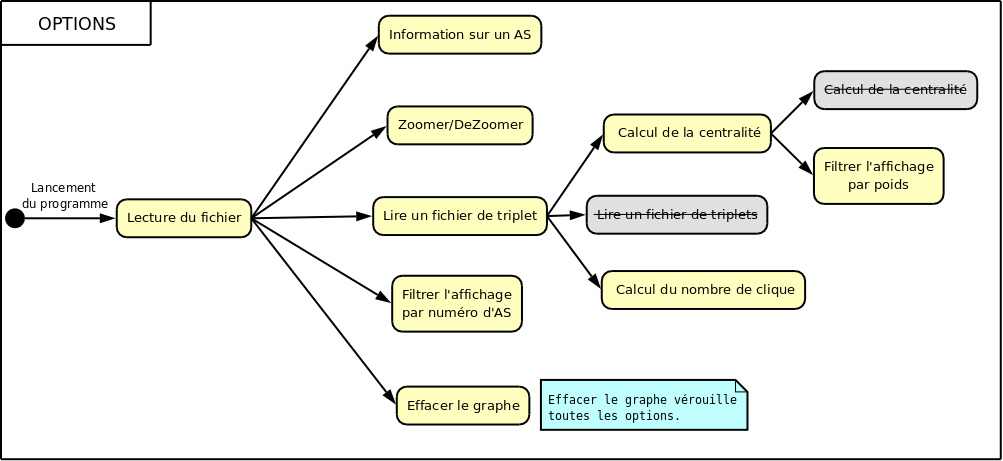
\includegraphics[width=\textwidth]{./seqMenu.png}}
}

\subsection{Rendu final}
\frame
{
\frametitle{Rendu final}
\only<1>
{
   \begin{center}
   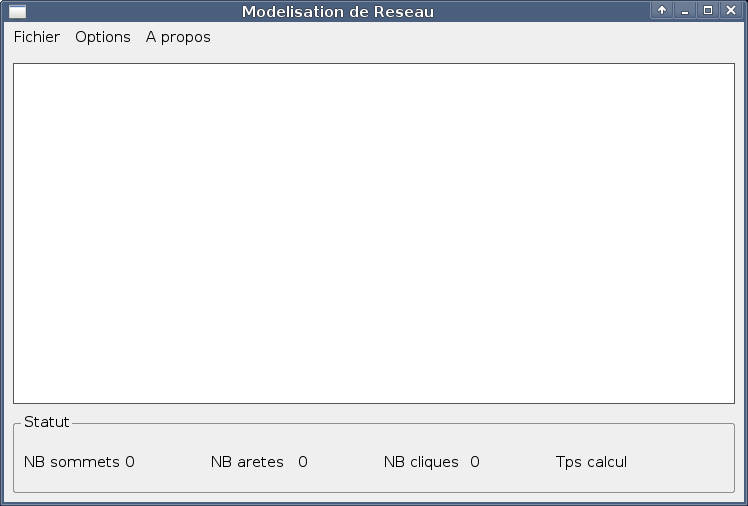
\includegraphics[width=0.9\textwidth]{ecran_programme.png}\\
   Ecran principal du programme
   \end{center}
}
\only<2>
{
   \begin{center}
   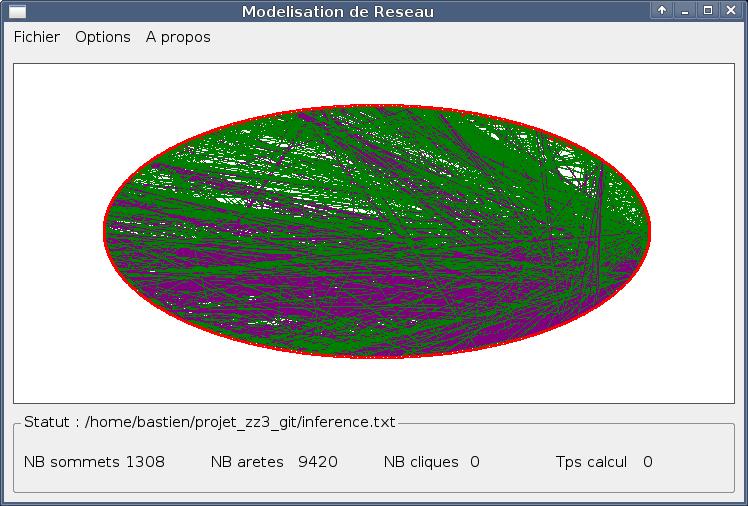
\includegraphics[width=0.9\textwidth]{ecran_graphe.png}\\
   Graphe charg\'e
   \end{center}
}
\only<3>
{
   \begin{center}
   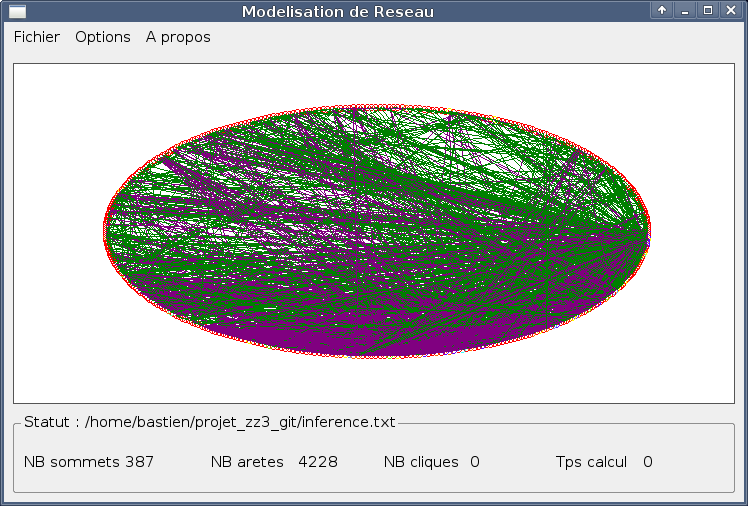
\includegraphics[width=0.9\textwidth]{ecran_graphe_nostubs.png}\\
   Stubs \'elimin\'es
   \end{center}
}
\only<4>
{
   \begin{center}
   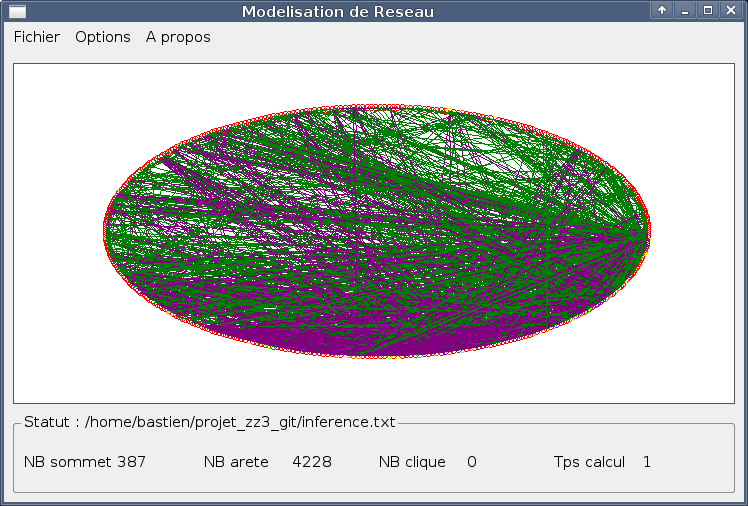
\includegraphics[width=0.9\textwidth]{ecran_graphe_centrality.png}\\
   Centralit\'e calcul\'ee
   \end{center}
}
\only<5>
{
   \begin{center}
   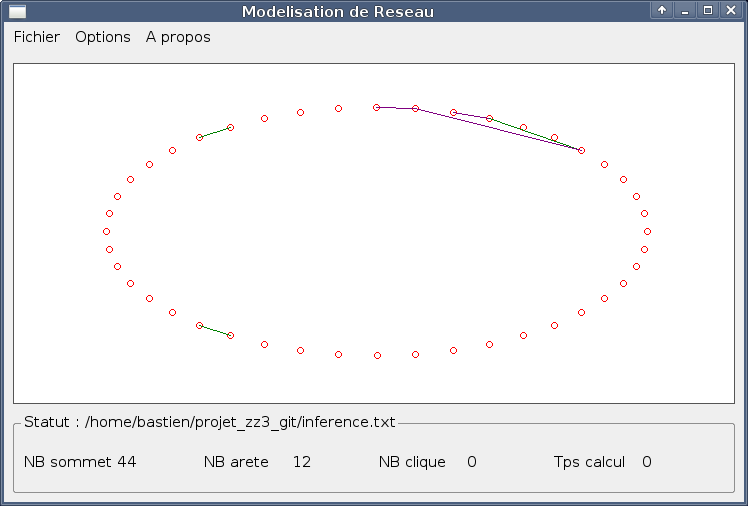
\includegraphics[width=0.9\textwidth]{ecran_graphe_filtre.png}\\
   Filtrage par num\'ero d'AS
   \end{center}
}
\only<6>
{
   \begin{center}
   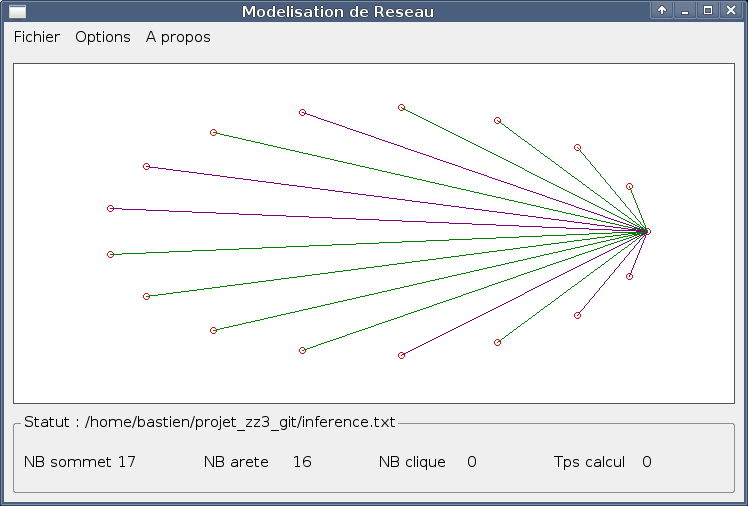
\includegraphics[width=0.9\textwidth]{ecran_graphe_zoom.png}\\
   Zoom sur un AS
   \end{center}
}
}